% Chapter Template

\chapter{Physical laws of Photon Simulation} % Main chapter title

\label{Chapter7} % Change X to a consecutive number; for referencing this chapter elsewhere, use \ref{ChapterX}

% %------------------------------------------------------------------------
% %	SECTION 1
% %------------------------------------------------------------------------

% \section{X-Ray Generation}

% about x-ray generation, filters the initial voltage and the beam, beam time

% about the abstraction of the x-ray beam to be uniformly distributed

% about the energy spectrum

% %------------------------------------------------------------------------
% %	SECTION 2
% %------------------------------------------------------------------------

% \section{About attenuation and scattering}

% about attenuation in materials: dependency on material and density

% about the different scattering types

% about the toal attenuation scattering coefficient

% about the detection of photons in pixels


This chapter introduces the physical and mathematical principles underlying the
simulation of X-ray imaging. Central to this is the modeling of individual
photon interactions with matter, including attenuation and scattering processes.
These interactions are inherently stochastic due to the quantum nature of
radiation-matter interactions. The stochastic nature of photons and their interactions with matter is modelled using monte Carlo methods of uniformly distributed values between 0 and 1, which are then transformed to follow the physical probability distributions relevant to the specific interactions being simulated. This approach allows for a realistic representation of photon transport and interaction within the imaging system.

\begin{figure}[H]
    \centering
    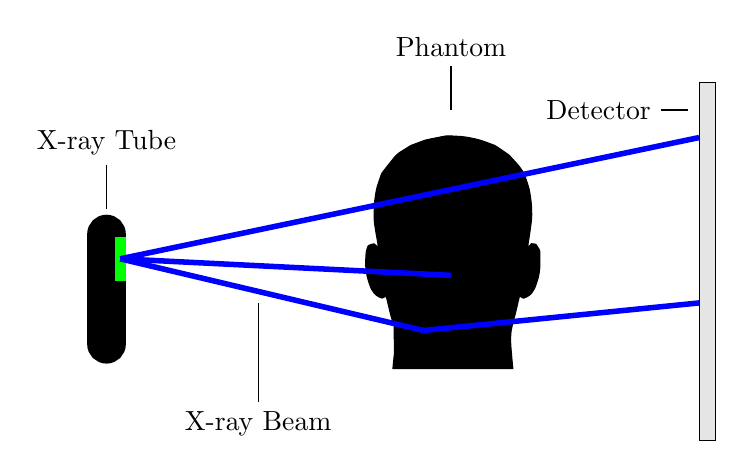
\begin{tikzpicture}[scale=.07]
        \draw[fill=black, rounded corners=5pt, line width=4] (-50,-40) rectangle (-45,-15);
        \draw[draw=green, line width=4] (-45,-18) -- (-45,-26);

        
        \draw[fill=gray!20] (60,10) rectangle (63,-55);
        
        \draw[fill=black]
        (349.5pt, -1.599976pt) .. controls (310.3pt, -9.299927pt) and (295pt,
        -12.79993pt) .. (287.5pt, -15.59998pt) -- (287.5pt, -15.59998pt) --
        (287.5pt, -15.59998pt) -- (287.5pt, -15.59998pt) .. controls (261.5pt,
        -25.09998pt) and (221.4pt, -40.19995pt) .. (219.6pt, -41.19995pt) --
        (219.6pt, -41.19995pt) -- (219.6pt, -41.19995pt) -- (219.6pt,
        -41.19995pt) .. controls (216.9pt, -42.59998pt) and (168.1pt, -73pt) ..
        (156.8pt, -80.29993pt) -- (156.8pt, -80.29993pt) -- (156.8pt,
        -80.29993pt) -- (156.8pt, -80.29993pt) .. controls (149.5pt, -85pt) and
        (146.4pt, -88pt) .. (138pt, -98.09998pt) -- (138pt, -98.09998pt) --
        (138pt, -98.09998pt) -- (138pt, -98.09998pt) .. controls (116.2pt,
        -124.2999pt) and (79.00001pt, -171.4999pt) .. (69.3pt, -185.4999pt) --
        (69.3pt, -185.4999pt) -- (69.3pt, -185.4999pt) -- (69.3pt, -185.4999pt)
        .. controls (67.3pt, -188.2999pt) and (50.10001pt, -239.1pt) .. (44.5pt,
        -258.4999pt) -- (44.5pt, -258.4999pt) -- (44.5pt, -258.4999pt) --
        (44.5pt, -258.4999pt) .. controls (40.3pt, -273.2pt) and (32.9pt,
        -320.7pt) .. (30.9pt, -345.9999pt) -- (30.9pt, -345.9999pt) -- (30.9pt,
        -345.9999pt) -- (30.9pt, -345.9999pt) .. controls (30.3pt, -353.9999pt)
        and (29.7pt, -374.2pt) .. (29.7pt, -390.9999pt) -- (29.7pt, -390.9999pt)
        -- (29.7pt, -390.9999pt) -- (29.7pt, -390.9999pt) .. controls (29.6pt,
        -418.2pt) and (29.9pt, -423.9pt) .. (32.2pt, -443.6pt) -- (32.2pt,
        -443.6pt) -- (32.2pt, -443.6pt) -- (32.2pt, -443.6pt) .. controls
        (33.7pt, -455.7pt) and (37.8pt, -482.1pt) .. (41.4pt, -502.1pt) --
        (41.4pt, -502.1pt) -- (41.4pt, -502.1pt) -- (41.4pt, -502.1pt) ..
        controls (49.10001pt, -544.8pt) and (51pt, -556.7pt) .. (51pt, -563.4pt)
        -- (51pt, -563.4pt) -- (51pt, -563.4pt) -- (51pt, -563.4pt) -- (51pt,
        -568.4pt) -- (51pt, -568.4pt) -- (40.6pt, -558.1pt) -- (40.6pt,
        -558.1pt) -- (40.6pt, -558.1pt) -- (40.6pt, -558.1pt) .. controls (29pt,
        -546.7pt) and (31.3pt, -547.4pt) .. (17.2pt, -551.1pt) -- (17.2pt,
        -551.1pt) -- (17.2pt, -551.1pt) -- (17.2pt, -551.1pt) .. controls
        (8.200001pt, -553.4999pt) and (0.500001pt, -557.3pt) .. (-1.499999pt,
        -560.3pt) -- (-1.499999pt, -560.3pt) -- (-1.499999pt, -560.3pt) --
        (-1.499999pt, -560.3pt) .. controls (-3.4pt, -563.2pt) and (-8.7pt,
        -580.7pt) .. (-10.5pt, -590.3pt) -- (-10.5pt, -590.3pt) -- (-10.5pt,
        -590.3pt) -- (-10.5pt, -590.3pt) .. controls (-11.3pt, -594.3pt) and
        (-12.5pt, -610.9pt) .. (-13.2pt, -627.3pt) -- (-13.2pt, -627.3pt) --
        (-13.2pt, -627.3pt) -- (-13.2pt, -627.3pt) -- (-14.4pt, -657.1pt) --
        (-14.4pt, -657.1pt) -- (-11.1pt, -683.8pt) -- (-11.1pt, -683.8pt) --
        (-11.1pt, -683.8pt) -- (-11.1pt, -683.8pt) .. controls (-7.4pt,
        -712.8pt) and (-5.099999pt, -723.2pt) .. (4.400002pt, -751.5pt) --
        (4.400002pt, -751.5pt) -- (4.400002pt, -751.5pt) -- (4.400002pt,
        -751.5pt) .. controls (14.6pt, -781.8pt) and (17.2pt, -786.9pt) ..
        (30.8pt, -803.4pt) -- (30.8pt, -803.4pt) -- (30.8pt, -803.4pt) --
        (30.8pt, -803.4pt) .. controls (38.2pt, -812.5pt) and (43.2pt, -816.3pt)
        .. (56.5pt, -823pt) -- (56.5pt, -823pt) -- (56.5pt, -823pt) -- (56.5pt,
        -823pt) .. controls (71.00001pt, -830.3pt) and (71.7pt, -830.3pt) ..
        (82.4pt, -823.5pt) -- (82.4pt, -823.5pt) -- (82.4pt, -823.5pt) --
        (82.4pt, -823.5pt) .. controls (89.2pt, -819.1pt) and (91.40001pt,
        -818.1pt) .. (92.10001pt, -819.2pt) -- (92.10001pt, -819.2pt) --
        (92.10001pt, -819.2pt) -- (92.10001pt, -819.2pt) .. controls
        (92.90001pt, -820.4pt) and (94.60001pt, -827.3pt) .. (107.5pt, -882pt)
        -- (107.5pt, -882pt) -- (107.5pt, -882pt) -- (107.5pt, -882pt) ..
        controls (115.6pt, -916.2pt) and (119.4pt, -930.2pt) .. (126.5pt,
        -952pt) -- (126.5pt, -952pt) -- (126.5pt, -952pt) -- (126.5pt, -952pt)
        -- (132.8pt, -971.5pt) -- (132.8pt, -971.5pt) -- (134pt, -1040.5pt) --
        (134pt, -1040.5pt) -- (135.1pt, -1109.5pt) -- (135.1pt, -1109.5pt) --
        (131.1pt, -1149.1pt) -- (131.1pt, -1149.1pt) -- (131.1pt, -1149.1pt) --
        (131.1pt, -1149.1pt) .. controls (128.8pt, -1170.9pt) and (127pt,
        -1189.7pt) .. (127pt, -1190.9pt) -- (127pt, -1190.9pt) -- (127pt,
        -1190.9pt) -- (127pt, -1190.9pt) -- (127pt, -1193pt) -- (127pt, -1193pt)
        -- (436.5pt, -1193pt) -- (436.5pt, -1193pt) -- (746.0001pt, -1193pt) --
        (746.0001pt, -1193pt) -- (745.5001pt, -1189.3pt) -- (745.5001pt,
        -1189.3pt) -- (745.5001pt, -1189.3pt) -- (745.5001pt, -1189.3pt) ..
        controls (744.0001pt, -1177.4pt) and (737.3pt, -1102pt) .. (735.4pt,
        -1075.5pt) -- (735.4pt, -1075.5pt) -- (735.4pt, -1075.5pt) -- (735.4pt,
        -1075.5pt) .. controls (733.4pt, -1047.1pt) and (733.9pt, -1024.6pt) ..
        (737.0001pt, -996pt) -- (737.0001pt, -996pt) -- (737.0001pt, -996pt) --
        (737.0001pt, -996pt) .. controls (739.5001pt, -972.6pt) and (740.1pt,
        -969.7pt) .. (748.0001pt, -946pt) -- (748.0001pt, -946pt) --
        (748.0001pt, -946pt) -- (748.0001pt, -946pt) .. controls (754.0001pt,
        -928.2pt) and (758.0001pt, -912.4pt) .. (771.1pt, -855.5pt) -- (771.1pt,
        -855.5pt) -- (771.1pt, -855.5pt) -- (771.1pt, -855.5pt) .. controls
        (778.4pt, -823.6pt) and (779.7pt, -819pt) .. (781.3pt, -819pt) --
        (781.3pt, -819pt) -- (781.3pt, -819pt) -- (781.3pt, -819pt) .. controls
        (782.0001pt, -819pt) and (785.3pt, -820.6pt) .. (788.6pt, -822.6pt) --
        (788.6pt, -822.6pt) -- (788.6pt, -822.6pt) -- (788.6pt, -822.6pt) ..
        controls (799.4pt, -829.3pt) and (799.7pt, -829.4pt) .. (804.4pt,
        -828pt) -- (804.4pt, -828pt) -- (804.4pt, -828pt) -- (804.4pt, -828pt)
        .. controls (810.3pt, -826.3pt) and (825.2001pt, -818.4pt) .. (831.8pt,
        -813.5pt) -- (831.8pt, -813.5pt) -- (831.8pt, -813.5pt) -- (831.8pt,
        -813.5pt) .. controls (839.3pt, -808.1pt) and (852.1pt, -791.1pt) ..
        (857.6pt, -779.5pt) -- (857.6pt, -779.5pt) -- (857.6pt, -779.5pt) --
        (857.6pt, -779.5pt) .. controls (862.1pt, -769.9pt) and (873.3pt,
        -736.7pt) .. (877.4pt, -721pt) -- (877.4pt, -721pt) -- (877.4pt, -721pt)
        -- (877.4pt, -721pt) .. controls (878.7001pt, -715.8pt) and (881.0001pt,
        -703.8pt) .. (882.4pt, -694.3pt) -- (882.4pt, -694.3pt) -- (882.4pt,
        -694.3pt) -- (882.4pt, -694.3pt) .. controls (884.9pt, -677.7pt) and
        (885.0001pt, -675.5pt) .. (885.0001pt, -632pt) -- (885.0001pt, -632pt)
        -- (885.0001pt, -632pt) -- (885.0001pt, -632pt) -- (885.0001pt,
        -586.8pt) -- (885.0001pt, -586.8pt) -- (881.0001pt, -576.7pt) --
        (881.0001pt, -576.7pt) -- (881.0001pt, -576.7pt) -- (881.0001pt,
        -576.7pt) .. controls (877.2001pt, -567.1pt) and (875.4pt, -564.2pt) ..
        (867.1pt, -554.2pt) -- (867.1pt, -554.2pt) -- (867.1pt, -554.2pt) --
        (867.1pt, -554.2pt) .. controls (863.5001pt, -549.8pt) and (862.9pt,
        -549.6pt) .. (848.9pt, -548.6pt) -- (848.9pt, -548.6pt) -- (848.9pt,
        -548.6pt) -- (848.9pt, -548.6pt) -- (842.3pt, -548.1pt) -- (842.3pt,
        -548.1pt) -- (834.4pt, -556.1pt) -- (834.4pt, -556.1pt) -- (834.4pt,
        -556.1pt) -- (834.4pt, -556.1pt) .. controls (830.1pt, -560.4999pt) and
        (825.3pt, -564.9999pt) .. (823.8pt, -566.1pt) -- (823.8pt, -566.1pt) --
        (823.8pt, -566.1pt) -- (823.8pt, -566.1pt) .. controls (821.4pt,
        -567.8pt) and (821.2001pt, -567.9pt) .. (821.6pt, -566.3pt) -- (821.6pt,
        -566.3pt) -- (821.6pt, -566.3pt) -- (821.6pt, -566.3pt) .. controls
        (823.1pt, -559.7pt) and (836.5001pt, -470.9pt) .. (839.0001pt,
        -450.9999pt) -- (839.0001pt, -450.9999pt) -- (839.0001pt, -450.9999pt)
        -- (839.0001pt, -450.9999pt) .. controls (843.3pt, -415.4pt) and
        (843.8pt, -406.4999pt) .. (842.9pt, -377.9999pt) -- (842.9pt,
        -377.9999pt) -- (842.9pt, -377.9999pt) -- (842.9pt, -377.9999pt) ..
        controls (841.8pt, -344.7pt) and (840.7001pt, -332.9pt) .. (835.9pt,
        -301.1pt) -- (835.9pt, -301.1pt) -- (835.9pt, -301.1pt) -- (835.9pt,
        -301.1pt) .. controls (830.4pt, -264.7999pt) and (831.3pt, -268.4pt) ..
        (815.5001pt, -219.9pt) -- (815.5001pt, -219.9pt) -- (815.5001pt,
        -219.9pt) -- (815.5001pt, -219.9pt) -- (805.2001pt, -188.4pt) --
        (805.2001pt, -188.4pt) -- (794.7pt, -171.9pt) -- (794.7pt, -171.9pt) --
        (794.7pt, -171.9pt) -- (794.7pt, -171.9pt) .. controls (788.8pt,
        -162.8999pt) and (780.5001pt, -151.2pt) .. (776.2pt, -146pt) --
        (776.2pt, -146pt) -- (776.2pt, -146pt) -- (776.2pt, -146pt) .. controls
        (769.8pt, -138.2pt) and (745.9pt, -112pt) .. (726.5001pt, -91.29993pt)
        -- (726.5001pt, -91.29993pt) -- (726.5001pt, -91.29993pt) --
        (726.5001pt, -91.29993pt) .. controls (724.3pt, -89pt) and (706.8pt,
        -76.69995pt) .. (687.5001pt, -63.8999pt) -- (687.5001pt, -63.8999pt) --
        (687.5001pt, -63.8999pt) -- (687.5001pt, -63.8999pt) -- (652.6pt,
        -40.69995pt) -- (652.6pt, -40.69995pt) -- (626.0001pt, -30.79993pt) --
        (626.0001pt, -30.79993pt) -- (626.0001pt, -30.79993pt) -- (626.0001pt,
        -30.79993pt) .. controls (585.2pt, -15.49988pt) and (570pt, -10.69995pt)
        .. (545pt, -5.499878pt) -- (545pt, -5.499878pt) -- (545pt, -5.499878pt)
        -- (545pt, -5.499878pt) .. controls (512.4pt, 1.200073pt) and (497pt,
        3.800049pt) .. (481.9pt, 5.000122pt) -- (481.9pt, 5.000122pt) --
        (481.9pt, 5.000122pt) -- (481.9pt, 5.000122pt) .. controls (460.8pt,
        6.600098pt) and (415.2pt, 9.000122pt) .. (408pt, 8.900024pt) -- (408pt,
        8.900024pt) -- (408pt, 8.900024pt) -- (408pt, 8.900024pt) .. controls
        (404.2pt, 8.800049pt) and (380pt, 4.500122pt) .. (349.5pt, -1.599976pt)
        -- cycle ;
        \draw[blue, line width=2] (-45,-22) -- (60,0);
        \draw[blue, line width=2] (-45,-22) -- (10,-35);
        \draw[blue, line width=2] (-45,-22) -- (15,-25);
        \draw[blue, line width=2] (10,-35) -- (60,-30);

        \draw (-47.5,-13) -- (-47.5,-5) node[above] {X-ray Tube};
        \draw (15,5) -- (15,13) node[above] {Phantom};
        \draw (58,5) -- (53,5) node [left] {Detector};
        \draw (-20,-30) -- (-20,-48) node[below] {X-ray Beam};
    \end{tikzpicture}
    \caption{Schematic illustration of photon transport in X-ray imaging.}
    \label{fig:photon_transport}
\end{figure}

In a typical simulation workflow, individual photons are emitted from the X-ray
tube and propagate through air before reaching the phantom. Upon entering the
phantom, they may interact with the material through scattering or absorption,
depending on the local composition of the tissue and photon energy. Only a
fraction of the photons will exit the phantom, continue their path through air,
and ultimately reach the detector, contributing to the final image formation.

The simulation framework described here forms the basis for all subsequent
analyses presented in this thesis.


%-------------------------------------------------------------------------------%	SECTION 2
\section{X-Ray Tube}
%-------------------------------------------------------------------------------

X-ray beams are generated within evacuated glass tubes containing several
critical components that convert electrical energy into X-ray photons and heat.
The X-ray tube acts as an energy converter, where the vast majority of the input
energy is transformed into heat and only a small fraction becomes useful
radiation. The following Figure~\ref{fig:xray_tube} illustrates the basic
construction of an X-ray tube as in \cite{poludniowski2022calculating}

\begin{figure}[htbp]
    \centering
    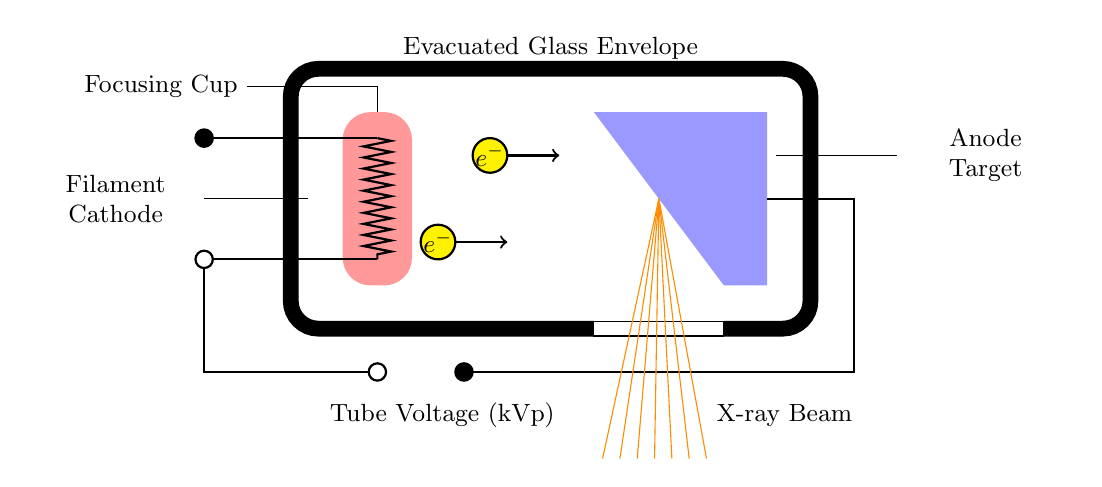
\begin{tikzpicture}[scale=1.1, every node/.style={font=\small}]
        % Glass envelope
        \draw[line width=2mm, rounded corners=10pt] (.5,-1.5) -- (-3,-1.5) -- (-3,1.5) -- (3,1.5) -- (3,-1.5) -- (2,-1.5);
        % Optional: dashed or lighter line to indicate the open section
        \draw (0.5,-1.415) rectangle (2,-1.585);
        \node[above] at (0,1.5) {Evacuated Glass Envelope};
        
        % Focusing Cup
        \draw[rounded corners=10pt, fill=red!40, draw=none] (-2.4,1) rectangle (-1.6,-1);
        \draw (-2,1) -- (-2,1.3) -- (-3.5,1.3) node [left] {Focusing Cup};

        % Filament (cathode)
        \draw[thick] (-4,.7) -- (-2,.7);
        \draw[thick, fill=black] (-4,.7) circle [radius=0.1];
        \draw[thick] (-4,-.7) -- (-2,-.7);
        \draw[thick] (-2,-2) -- (-4,-2) -- (-4,-.7);
        \draw[thick, fill=white] (-4,-.7) circle [radius=0.1];
        \draw[thick, decorate, decoration={zigzag, segment length=4pt, 
        amplitude=5pt}] (-2,.7) -- (-2,-.7);
        \draw (-2.8,0) -- (-4,0) node[left, align=center, text width=2cm] {Filament\\Cathode};

        % Anode Target
        \draw[fill=blue!40, draw=none] (.5,1) -- (2.5,1) -- (2.5,-1) -- (2,-1) -- cycle;
        \draw (2.6,.5) -- (4,.5) node[right, align=center, text width=2cm] {Anode\\Target};

        % Anode Voltage
        \draw[thick] (2.5,0) -- (3.5,0) -- (3.5,-2) -- (-1,-2);
        \draw[thick, fill=black] (-1,-2) circle [radius=0.1];
        \draw[thick, fill=white] (-2,-2) circle [radius=0.1];
        \node[below, align=center, text height=.5cm] at (-1.25,-2) {Tube Voltage (kVp)};

        % Electrons
        \draw[thick,->] (-1.3,-.5) -- (-.5,-.5);
        \draw[thick, fill=yellow] (-1.3,-.5) circle [radius=0.2] node[font=\small] {$e^{\text{-}}$};
        \draw[thick,->] (-.7,.5) -- (.1,.5);
        \draw[thick, fill=yellow] (-.7,.5) circle [radius=0.2] node[font=\small] {$e^{\text{-}}$};

        % Photon Beam
        \draw[orange!90!yellow] (.6,-3) -- (1.25,0);
        \draw[orange!90!yellow] (.8,-3) -- (1.25,0);
        \draw[orange!90!yellow] (1,-3) -- (1.25,0);
        \draw[orange!90!yellow] (1.2,-3) -- (1.25,0);
        \draw[orange!90!yellow] (1.4,-3) -- (1.25,0);
        \draw[orange!90!yellow] (1.6,-3) -- (1.25,0);
        \draw[orange!90!yellow] (1.8,-3) -- (1.25,0);
        \node[right, below, align=center, text height=.5cm] at (2.7,-2) {X-ray Beam};
    \end{tikzpicture}
    \caption{Schematic of an X-ray tube.}
    \label{fig:xray_tube}
\end{figure}


\subsection{Photon Generation}

To capture this randomness, Monte Carlo methods
are employed. In such simulations, random numbers—typically sampled uniformly
from the interval $[0,1]$ are transformed into physically meaningful
quantities according to the relevant probability distributions. This
probabilistic modeling enables realistic simulation of photon transport and
forms the basis for the analyses presented in this thesis.



The key components are:

\begin{itemize}
    \item \textbf{Filament (Cathode):} A tungsten wire filament serves as the
    electron source through thermionic emission. When a current of approximately
    3-6\,A passes through it, the filament reaches incandescence, releasing
    electrons from its surface. These free electrons form a cloud near the
    cathode until they are accelerated toward the anode by the applied high
    voltage.

    \item \textbf{Focusing Cup:} The filament is embedded in a negatively
    charged, nickel-made focusing cup. Its function is to electrostatically
    shape and direct the electron stream toward the anode’s focal spot, thereby
    influencing the resolution and size of the resulting X-ray beam.

    \item \textbf{Anode Target:} The anode consists of a tungsten target, often
    embedded in a copper support. Tungsten is used for its high atomic number
    and melting point, enhancing X-ray production and durability. The copper
    base improves heat dissipation. Typically, less than 1\% of the electron
    energy is converted into X-rays, with the remainder generating heat that
    must be effectively managed.

    \item \textbf{Evacuated Glass Envelope:} All components are sealed within a
    borosilicate glass or metal-ceramic housing evacuated to a low pressure
    (typically $10^{-5}$ to $10^{-7}$\,hPa). The vacuum allows unimpeded
    electron flow and prevents arcing. The housing is usually immersed in
    insulating oil to provide thermal and electrical isolation.
\end{itemize}

When high-energy electrons strike the tungsten target, X-ray photons are
produced through two primary mechanisms:

\begin{itemize}
    \item \textbf{Bremsstrahlung (Braking Radiation):} This accounts for
    approximately 80\% of X-ray production. When electrons pass close to
    tungsten nuclei, they are decelerated by the electrostatic attraction,
    causing them to lose kinetic energy that is emitted as X-ray photons. This
    process produces a continuous spectrum of X-ray energies from near zero up
    to the maximum electron energy.

    \item \textbf{Characteristic Radiation:} This occurs when high-energy
    electrons knock inner shell electrons from tungsten atoms. When outer shell
    electrons drop down to fill these vacancies, they emit X-rays with discrete,
    characteristic energies specific to tungsten. Therefore peaks are occuring
    at the difference of the binding energies of the electron shells. For
    reference, the atomic model of tungsten is given in
    Figure~\ref{fig:tungsten_atomic_model} and the approximate binding energies
    of the electron shells in Table~\ref{tab:tungsten_binding_energies}.

    \begin{table}[!h]
        \centering
        \begin{tabular}{cc}
            \toprule
            \textbf{Shell / Subshell} & \textbf{Binding Energy (keV)} \\
            \midrule
            K        & 69.5 \\
            L$_1$    & 12.1 \\
            L$_2$    & 11.5 \\
            L$_3$    & 10.2 \\
            M$_1$    & 2.82 \\
            M$_2$    & 2.30 \\
            M$_3$    & 2.15 \\
            N$_1$    & 0.43 \\
            N$_2$    & 0.32 \\
            N$_3$    & 0.22 \\
            \bottomrule
        \end{tabular}
        \caption{Approximate Electron Binding Energies of Tungsten (W, Z = 74)}
        \label{tab:tungsten_binding_energies}
    \end{table}

    % TODO: W und Z sollten als Abkürzungen in \ac{acronym} definiert werden

    \begin{figure}
        \centering
        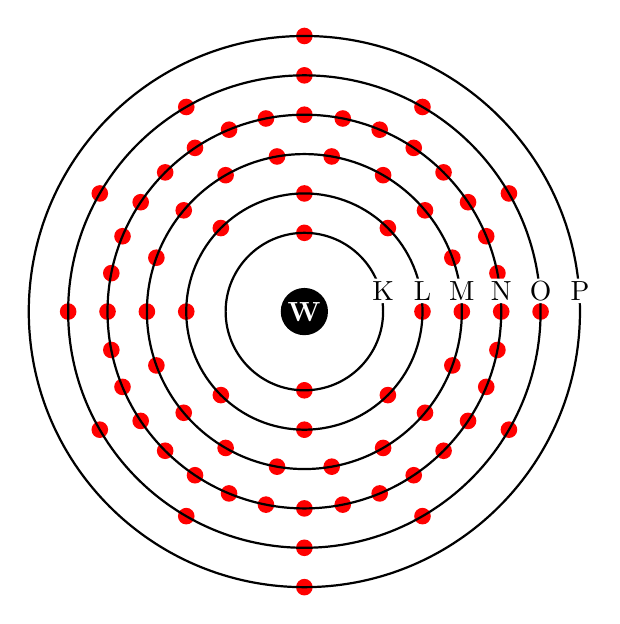
\begin{tikzpicture}[scale=1]
            % Kern
            \fill[black] (0,0) circle (0.3);
            \node at (0,0) [white] {\textbf{W}};

            % Elektronen (vereinfacht verteilt)
            % K-Schale: 2
            \foreach \angle in {90, 270} {
                \fill[color=red] (0,0) ++(\angle:1) circle (3pt);
            }

            % L-Schale: 8
            \foreach \angle in {0, 45, 90, 135, 180, 225, 270, 315} {
                \fill[color=red] (0,0) ++(\angle:1.5) circle (3pt);
            }

            % M-Schale: 18
            \foreach \angle in {0, 20, 40, 60, 80, 100, 120, 140, 160, 180, 200, 220, 240, 260, 280, 300, 320, 340} {
                \fill[color=red] (0,0) ++(\angle:2cm) circle (3pt);
            }

            % N-Schale: 32
            \foreach \angle in {0,11.25,...,348.75} {
                \fill[color=red] (0,0) ++(\angle:2.5cm) circle (3pt);
            }

            % O-Schale: 12
            \foreach \angle in {0,30,...,330} {
                \fill[color=red] (0,0) ++(\angle:3cm) circle (3pt);
            }

            % P-Schale: 2
            \foreach \angle in {90, 270} {
                \fill[color=red] (0,0) ++(\angle:3.5cm) circle (3pt);
            }
            
            % Schalen
            \foreach \radius/\label in {
                1/K,
                1.5/L,
                2/M,
                2.5/N,
                3/O,
                3.5/P
            } {
                \draw[thick] (0,0) circle (\radius);
                \node[above, fill=white, inner sep=1pt, rounded corners=1pt] at (\radius, 0.1) {\label};
            }
        \end{tikzpicture}
        \caption{Bohr model of the tungsten atom (W, Z = 74) with electron shells and subshells.}
        \label{fig:tungsten_atomic_model}
    \end{figure}

    In Table~\ref{tab:tungsten_binding_energies} only binding energies of the K,
    L and M shells are given, since these are the most relevant for X-ray
    production. The binding energies of the N shell and higher shells are
    negligible in this context due to their low binding energies.   
    
\end{itemize}

Although it is not necessary to understand every technical detail of the X-ray
apparatus for the purposes of simulation, I found it important to briefly
present the fundamental working principles of the X-ray tube. This background
allows one to appreciate how key simulation parameters for photon generation -
specifically the tube voltage and the cathode material - influence the resulting
X-ray spectrum and photon behavior.

Figure~\ref{fig:spectrum100kvp} below shows an resulting energy spectrum for an
X-ray tube with a tungsten cathode operated at 100 kVp. It illustrates the
resulting distribution of photon energies, which is shaped by both the material
and the applied voltage. The intensity of the different photon energies is
measured in \emph{spectral fluence} in
\si{\per\square\centi\meter\per\kilo\electronvolt}, which describes the number
of X-ray photons per unit area per unit energy interval. It certainly shows the
two components of the X-ray spectrum: the continuous bremsstrahlung spectrum and
the characteristic radiation peaks:

\begin{figure}[H]
    \centering
    \includegraphics[width=0.8\textwidth]{Figures/spectrum_without_filter.png}
    \caption{X-ray spectrum for a tungsten cathode at 100 kVp showing the
    continuous bremsstrahlung spectrum and characteristic peaks. Build with
    \emph{SpekPy} \cite{spekpy}}
    \label{fig:spectrum100kvp}
\end{figure}


\subsection{Filter}
\label{sec:filter}

Low energy X-ray photons contribute little to image formation but significantly
increase patient dose. Therefore, X-ray tubes are often equipped with filters to
selectively attenuate these low-energy photons while allowing higher-energy
photons to pass through. This process, known as beam hardening, improves image
quality by reducing scatter and enhancing contrast. Common filter materials
include aluminum, copper, and molybdenum, which are chosen based on their atomic
number and thickness to effectively absorb low-energy photons while minimizing
the impact on higher-energy photons \cite{poludniowski2022calculating}.

As can be seen in Figure~\ref{fig:xray_tube_with_filter}, the filter is placed
between the TODO:WHAT???? at the margin of the X-ray tube. Followingly X-rays pass through the
filter before reaching the patient.

\begin{figure}[H]
    \centering
    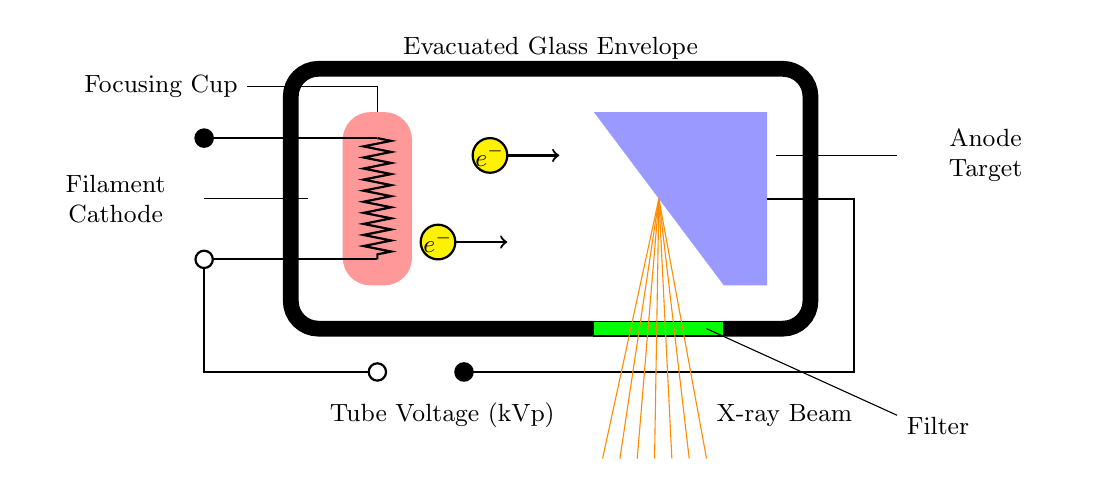
\begin{tikzpicture}[scale=1.1, every node/.style={font=\small}]
        % Glass envelope
        \draw[line width=2mm, rounded corners=10pt] (.5,-1.5) -- (-3,-1.5) -- (-3,1.5) -- (3,1.5) -- (3,-1.5) -- (2,-1.5);
        % Optional: dashed or lighter line to indicate the open section
        \draw[fill=green] (0.5,-1.415) rectangle (2,-1.585);
        \node[above] at (0,1.5) {Evacuated Glass Envelope};
        
        % Focusing Cup
        \draw[rounded corners=10pt, fill=red!40, draw=none] (-2.4,1) rectangle (-1.6,-1);
        \draw (-2,1) -- (-2,1.3) -- (-3.5,1.3) node [left] {Focusing Cup};

        % Filament (cathode)
        \draw[thick] (-4,.7) -- (-2,.7);
        \draw[thick, fill=black] (-4,.7) circle [radius=0.1];
        \draw[thick] (-4,-.7) -- (-2,-.7);
        \draw[thick] (-2,-2) -- (-4,-2) -- (-4,-.7);
        \draw[thick, fill=white] (-4,-.7) circle [radius=0.1];
        \draw[thick, decorate, decoration={zigzag, segment length=4pt, 
        amplitude=5pt}] (-2,.7) -- (-2,-.7);
        \draw (-2.8,0) -- (-4,0) node[left, align=center, text width=2cm] {Filament\\Cathode};

        % Anode Target
        \draw[fill=blue!40, draw=none] (.5,1) -- (2.5,1) -- (2.5,-1) -- (2,-1) -- cycle;
        \draw (2.6,.5) -- (4,.5) node[right, align=center, text width=2cm] {Anode\\Target};

        % Anode Voltage
        \draw[thick] (2.5,0) -- (3.5,0) -- (3.5,-2) -- (-1,-2);
        \draw[thick, fill=black] (-1,-2) circle [radius=0.1];
        \draw[thick, fill=white] (-2,-2) circle [radius=0.1];
        \node[below, align=center, text height=.5cm] at (-1.25,-2) {Tube Voltage (kVp)};

        % Electrons
        \draw[thick,->] (-1.3,-.5) -- (-.5,-.5);
        \draw[thick, fill=yellow] (-1.3,-.5) circle [radius=0.2] node[font=\small] {$e^{\text{-}}$};
        \draw[thick,->] (-.7,.5) -- (.1,.5);
        \draw[thick, fill=yellow] (-.7,.5) circle [radius=0.2] node[font=\small] {$e^{\text{-}}$};

        % Photon Beam
        \draw[orange!90!yellow] (.6,-3) -- (1.25,0);
        \draw[orange!90!yellow] (.8,-3) -- (1.25,0);
        \draw[orange!90!yellow] (1,-3) -- (1.25,0);
        \draw[orange!90!yellow] (1.2,-3) -- (1.25,0);
        \draw[orange!90!yellow] (1.4,-3) -- (1.25,0);
        \draw[orange!90!yellow] (1.6,-3) -- (1.25,0);
        \draw[orange!90!yellow] (1.8,-3) -- (1.25,0);
        \node[right, below, align=center, text height=.5cm] at (2.7,-2) {X-ray Beam};
        \draw (1.8,-1.5) -- (4,-2.5) node[right, align=center, text height=.5cm] {Filter};
    \end{tikzpicture}
    \caption{Schematic of an X-ray tube with Filter.}
    \label{fig:xray_tube_with_filter}
\end{figure}

Throughout this thesis, a filter consisting of
$0.4$ \si{\milli\meter} Tin (Sn) is used for the simulations. This filter is chosen to represent a
realistic X-ray tube filter that is commonly used in clinical
practice \cite{steidel2022dose}. The resulting spectrum is shown in
Figure~\ref{fig:spectrum100kvp_with_filter}.

\begin{figure}[H]
    \centering
    \includegraphics[width=0.8\textwidth]{Figures/spectrum_with_filter.png}
    \caption{X-ray spectrum for a tungsten cathode at $100$ \si{\kilo\voltpeak}
    with a $0.4$ \si{\milli\meter} showing the continuous bremsstrahlung
    spectrum and characteristic peaks. Build with \emph{SpekPy} \cite{spekpy}}
    \label{fig:spectrum100kvp_with_filter}
\end{figure}


%-------------------------------------------------------------------------------
%	SECTION 3
\section{Photon Generation}
%-------------------------------------------------------------------------------

In the context of Monte Carlo simulations, photons are generated from the X-ray
tube source, which is typically modeled as a point source emitting photons
within a conical beam. The emission cone is defined by a half-angle $\Theta$,
which determines the angular distribution of emitted photons. -- The emitted photons are characterized by two key properties: their direction and
energy. 

\subsection*{Photon Energy}
The photon energy is sampled from the X-ray tube spectrum as described in
Section~\ref{sec:filter}. In the simulations referenced in this thesis the
spectra are generated utilizing \emph{SpekPy} \cite{spekpy,
poludniowski2021spekpy}. The energies of the resulting photons are sampled via
inverse transform sampling from the normalized spectrum.

Inverse transform sampling \cite{muller2012monte} is a method to generate random samples from a target distribution using uniformly distributed random variables, such as those generated by a Quasi-Monte Carlo sequence.

\begin{definition}[Inverse Transform Sampling]\ \\
    \label{def:inverse_transform_sampling}
    Let $F_X: \mathbb{R} \to [0,1]$ be the cumulative distribution function (CDF) of a continuous, strictly increasing random variable $X$. The method of \emph{inverse transform sampling} generates a realization of $X$ by the following procedure:

    \begin{enumerate}
        \item Generate a sample $U$ from the uniform distribution on the unit interval, i.e., $U \sim \mathcal{U}(0,1)$.
        \item Compute the value $X := F_X^{-1}(U)$, where $F_X^{-1}$ denotes the inverse of the CDF $F_X$.
    \end{enumerate}
\end{definition}

\begin{theorem}\ \\
Let $F_X$ be a continuous and strictly increasing cumulative distribution function, and let $U \sim \mathcal{U}(0,1)$. Then the random variable
\[
X := F_X^{-1}(U)
\]
has cumulative distribution function $F_X$, i.e.,
\[
\mathbb{P}(X \leq x) = F_X(x), \quad \text{for all } x \in \mathbb{R}.
\]
\end{theorem}

\begin{proof}\ \\
Since $F_X$ is continuous and strictly increasing, its inverse $F_X^{-1}$ exists. For any $x \in \mathbb{R}$, we compute:

\[
\mathbb{P}(X \leq x) = \mathbb{P}(F_X^{-1}(U) \leq x)
= \mathbb{P}(U \leq F_X(x)) \quad  \underset{\text{decreasing}}{\overset{\text{since } F_X \text{ is strictly}}{=}} F_X(x),
\]

because \( U \sim \mathcal{U}(0,1) \) and thus \( \mathbb{P}(U \leq u) = u \) for all \( u \in [0,1] \). This shows that \( X \) has CDF \( F_X \).
\end{proof}


\subsection*{Photon Direction}
The direction of each emitted photon is sampled uniformly within a conical
emission cone defined by the half-angle $\Theta$. For the simulation a spherical alignment of the X-ray tube is assumed, such that the beam is oriented along the vector $\vec{v} = (v_1,v_2,v_3)$ in the Cartesian coordinate system.

Followingly, the direction of the emitted photon is sampled based on two random
values $u_1, u_2 \in [0,1)$ as follows:
\begin{enumerate}
    \item Sample a random angle $\theta$ uniformly from the interval $[0,
    \Theta]$ with $u_1$:
    $$\theta = u_1 \cdot \Theta$$
    \item Sample a random azimuthal angle $\phi$ uniformly from the interval
    $[0, 2\pi)$ with $u_2$:
    $$\phi = u_2 \cdot 2\pi$$
    \item Compute the direction vector $\vec{d}$ of the photon as:
    $$\vec{d} = (\sin(\theta) \cos(\phi), \sin(\theta) \sin(\phi),
    \cos(\theta))$$
\end{enumerate}


% ------------------------------------------------------------------------------
\section{Scattering and Attenuation}
%-------------------------------------------------------------------------------

This section provides the basic concepts of photon interaction with matter. The
interaction relevant for medical imaging results in a reduction of radiation
intensity, which corresponds to a decreased number of photons reaching the
detector. Hereby X-ray photons may be fully absorbed by \emph{photoelectric absorption} or undergo either \emph{elastic scattering} (Rayleigh) or \emph{inelastic scattering} (Compton) as they interact with matter.

The attenuation of X-ray photons arises from physical processes that alter their
number, direction, or energy as they interact with matter. These interactions
occur at the level of individual photons and are highly dependent on the photon
energy. This section presents an overview of the primary interaction mechanisms
relevant to attenuation like in \cite{medicalImagingSystemsIntro2019:}.

For correctness, in the simmulations it is further assumed that the X-ray
photons are propagating through vacuum before entering and after exiting the
phantom. Usually the tissues are surrounded by air, which has a negligible
effect on the photon transport.

\begin{figure}
    \centering
    \begin{minipage}[t]{0.45\textwidth}
        \raggedright
        \begin{tikzpicture}[scale=.8]
            \draw[decorate, decoration=snake, {Latex[scale=1.5]}-, shorten <=-10] (2.5,2.3) -- (-2.5,2.3) node[left] {\small$\gamma$};
            \fill[black] (0,0) circle (0.3);
            \foreach \angle in {90, 270} {
                \fill[color=blue] (0,0) ++(\angle:1) circle (3pt);
            }
            \foreach \angle in {0, 45, 90, 135, 180, 225, 270, 315} {
                \fill[color=blue] (0,0) ++(\angle:1.5) circle (3pt);
            }
            \foreach \angle in {0, 40, 80, 120, 160, 200, 240, 280, 320} {
                \fill[color=blue] (0,0) ++(\angle:2cm) circle (3pt);
            }
            \foreach \radius in {1,1.5,2}
            {
                \draw[thick] (0,0) circle (\radius);
            }
            \node[below, font=\large] at (0,-2.5) {No Interaction};
        \end{tikzpicture}
    \end{minipage}
    \begin{minipage}[t]{0.45\textwidth}
        \raggedleft
        \begin{tikzpicture}[scale=.8]
            \draw[decorate, decoration=snake, segment length=2mm, {Latex[scale=1.5]}-, shorten <=-10] (2.5,-.15) -- (.25,-.7) -- (-2.5,-.25) node[left] {\small$\gamma$};
            \fill[black] (0,0) circle (0.3);
            \foreach \angle in {90, 270} {
                \fill[color=blue] (0,0) ++(\angle:1) circle (3pt);
            }
            \foreach \angle in {0, 45, 90, 135, 180, 225, 270, 315} {
                \fill[color=blue] (0,0) ++(\angle:1.5) circle (3pt);
            }
            \foreach \angle in {0, 40, 80, 120, 160, 200, 240, 280, 320} {
                \fill[color=blue] (0,0) ++(\angle:2cm) circle (3pt);
            }
            \foreach \radius in {1,1.5,2}
            {
                \draw[thick] (0,0) circle (\radius);
            }
            \node[below, font=\large] at (0,-2.5) {Rayleigh Scattering};
        \end{tikzpicture}
    \end{minipage}
    \par\vspace{2em}
    \begin{minipage}[t]{0.45\textwidth}
        \raggedright
        \begin{tikzpicture}[scale=.8]
            \draw[decorate, decoration=snake] (0,1) -- (-2.5,2.1) node[left] {\small$\gamma$};
            \draw[thick] [thick, -{Latex[scale=1.5]}, shorten >=5] (0,1) --
            (2.5, .7) node[draw, circle, fill=black, minimum size=5pt, inner
            sep=0pt] {} node[xshift=10pt, yshift=2pt] {\small$e^\text{-}$};
            \foreach \angle in {90, 270} {
                \fill[color=blue] (0,0) ++(\angle:1) circle (3pt);
            }
            \foreach \angle in {0, 45, 90, 135, 180, 225, 270, 315} {
                \fill[color=blue] (0,0) ++(\angle:1.5) circle (3pt);
            }
            \foreach \angle in {0, 40, 80, 120, 160, 200, 240, 280, 320} {
                \fill[color=blue] (0,0) ++(\angle:2cm) circle (3pt);
            }
            \foreach \radius in {1,1.5,2}
            {
                \draw[thick] (0,0) circle (\radius);
            }
            \node[below, font=\large] at (0,-2.5) {Photoelectric Absorption};
        \end{tikzpicture}
    \end{minipage}
    \begin{minipage}[t]{0.45\textwidth}
        \raggedleft
        \begin{tikzpicture}[scale=.8]
            \draw[decorate, decoration=snake, segment length=2mm] (.3,-2) --
            (-2.5,-2) node[left] {\small$\gamma$};
            \draw[decorate, decoration=snake, segment length=4mm, -{Latex[scale=1.5]}, shorten >=-6] (.3,-2) -- (2.0,-1.5);
            \draw[thick, -{Latex[scale=1.5]}, shorten >=5] (.3,-2) -- (2.5,-2.5)
            node[draw, circle, fill=black, minimum size=5pt, inner sep=0pt] {}
            node[xshift=10pt, yshift=2pt] {\small$e^\text{-}$};
            \fill[black] (0,0) circle (0.3);
            \foreach \angle in {90, 270} {
                \fill[color=blue] (0,0) ++(\angle:1) circle (3pt);
            }
            \foreach \angle in {0, 45, 90, 135, 180, 225, 270, 315} {
                \fill[color=blue] (0,0) ++(\angle:1.5) circle (3pt);
            }
            \foreach \angle in {0, 40, 80, 120, 160, 200, 240, 280, 320} {
                \fill[color=blue] (0,0) ++(\angle:2cm) circle (3pt);
            }
            \foreach \radius in {1,1.5,2}
            {
                \draw[thick] (0,0) circle (\radius);
            }
            \node[below, font=\large] at (0,-2.5) {Compton Scattering};
        \end{tikzpicture}
    \end{minipage}
    % \begin{minipage}[t]{0.45\textwidth}
    %     \centering
    %     \begin{tikzpicture}[scale=.8]
    %         \draw[decorate, decoration=snake, segment length=2mm] (0,-.3) --
    %         (-2.5,-.3) node[left] {\small$\gamma$};
    %         \draw[thick, -{Latex[scale=1.5]}, shorten >=5] (0,-.3) -- (2.5,1)
    %         node[draw, circle, fill=black, minimum size=5pt, inner sep=0pt] {}
    %         node[xshift=10pt, yshift=2pt] {\small$e^\text{-}$};
    %         \draw[thick, -{Latex[scale=1.5]}, shorten >=5] (0,-.3) -- (2.5,-1.3)
    %         node[draw, circle, fill=black, minimum size=5pt, inner sep=0pt] {}
    %         node[xshift=10pt, yshift=2pt] {\small$e^\text{-}$};
    %         \fill[black] (0,0) circle (0.3);
    %         \foreach \angle in {90, 270} {
    %             \fill[color=blue] (0,0) ++(\angle:1) circle (3pt);
    %         }
    %         \foreach \angle in {0, 45, 90, 135, 180, 225, 270, 315} {
    %             \fill[color=blue] (0,0) ++(\angle:1.5) circle (3pt);
    %         }
    %         \foreach \angle in {0, 40, 80, 120, 160, 200, 240, 280, 320} {
    %             \fill[color=blue] (0,0) ++(\angle:2cm) circle (3pt);
    %         }
    %         \foreach \radius in {1,1.5,2}
    %         {
    %             \draw[thick] (0,0) circle (\radius);
    %         }
    %         \node[below, font=\large] at (0,-2.5) {Pair Production};
    %     \end{tikzpicture}
    % \end{minipage}
    \caption{Principles from photon interaction with matter similar to \cite[Chap. 7]{medicalImagingSystemsIntro2019:}}
    \label{fig:tungsten_atomic_model}
\end{figure}

\subsection{Free Path Length}

All mentioned interaction processes - the photoelectric effect, Compton
scattering and Rayleigh scattering - are probabilistic in nature. The according
attenuation coefficients $\mu$ characterizes the extend of the beam being
reduced by its according effect, when passing through the material, in \si{\square\centi\metre\per\gram}. For the
simulation of photons, the attenuation coefficients are dependend on the
according energy $E$ of the photon and the material at spherical location $x$ of
the photon. The coefficients are summarized in
Table~\ref{tab:attenuation_coefficients}.

\begin{table}[H]
    \centering
    \begin{tabular}{lcc}
        \toprule
        \textbf{Interaction Type} & \textbf{Attenuation Coefficient} \\
        \midrule
        Photoelectric Effect & $\mu_{\text{PE}}(x,E)$ \\
        Rayleigh Scattering & $\mu_{\text{RS}}(x,E)$ \\
        Compton Scattering & $\mu_{\text{CS}}(x,E)$ \\
        \bottomrule
    \end{tabular}
    \caption{Attenuation coefficients for different photon interaction mechanisms.}
    \label{tab:attenuation_coefficients}
\end{table}

The linear attenuation coefficient $\mu(x,E)$ is the sum of the individual
attenuation coefficients of the interaction coefficients:

$$\mu(x,E) = \mu_{\text{PE}}(x,E) + \mu_{\text{RS}}(x,E) +
\mu_{\text{CS}}(x,E)$$

When an X-ray photon eneters the phantom two main effects are considered:
\begin{itemize}
    \item \textbf{Attenuation:} The photon may be absorbed or Scattered.
    \item \textbf{No Interaction:} The photon may pass through the phantom
    without any interaction.
\end{itemize}

The \emph{free path length} $t$ of a photon describes the distance a photon takes to traverse through the phantom before it interacts with matter. Supposing the phantoms location is $x$ and the photon is traveling in the unit direction $\vec{v}$, as in \cite{qmcXray2023} the free path length $t$ follows the distribution given by:

$$t \sim \mu(x,E)\exp\bigg[-\int_{0}^{t}{\mu(x+s\cdot\vec{v})}\bigg]$$

\textcolor{red}{Check: nach dem paper müsste $\mu$ abhängig vom Endpunkt sein.}

The free path length $t$ is constraint by the maximum distance $c$ ($0\leq t\leq
c$) to the next exit point of the phantom along the ray with direction
$\vec{v}$. After leaving the phantom, we assume the photon is reaching the
detector or leaving the simulation domain.

The probability of the photon to leave the phantom unaltered is
described by the \emph{escape probability} $\mathcal{P}$ of a photon at a given
position $A$ with unit direction $\vec{v}$ and energy $E$ as in
\cite{qmcXray2023}:

$$\mathcal{P}(x, \vec{v}, E) = \exp \bigg[ -\int\limits_{0}^{c}{\mu(x+t\vec{v}, E)} dt \bigg],$$

\begin{figure}[H]
    \centering
    \begin{tikzpicture}[scale=1]
        \draw[color=gray, fill=gray!30] plot[smooth cycle] coordinates {(-2,0) (-2.5,1.5) (0,3) (3,1.5) (4,-1) (3,-2) (-2,-2.5)};
        \filldraw[fill=black] (-5,.5) circle (4pt) node[above, inner sep=7pt] {$S$};
        \node[below, inner sep=7pt] at (-3.5,.25) {$\vec{v}$};
        \draw[thick] (-5,.5) -- (-2,0);
        \filldraw[fill=black] (-2,0) circle (4pt) node[above, inner sep=7pt] {$A_0$};
        \draw[thick] (-2,0) -- (4,-1);
        \filldraw[fill=black] (4,-1) circle (4pt) node[above, inner sep=7pt] {$C$};
        \draw[thick, -{Latex[scale=1.5]}] (4,-1) -- (7,-1.5);

        % \node[above] at (-.5,.5) {$A_0$};
    \end{tikzpicture}
    \caption{Illustration of the entry and exit point of the ray of a photon without interaction.}
    \label{fig:exit_point}
\end{figure}

\textcolor{green}{Todo: Image illustrating the entry and exit point of a ray without interaction.}


\subsection{Compton Scattering}
\emph{Compton scattering} is the most dominant interaction mechanism for X-ray
photons in tissue \cite[Chap. 7]{medicalImagingSystemsIntro2019:}. It occurs
when an X-ray photon collides with a loosely bound outer shell electron,
resulting in a transfer of energy and momentum. The photon is scattered at an
angle and its energy is reduced, while the electron is ejected from the atom.